% !TEX root = ../main.tex
\chapter*{Analysis}
\label{Analysis}

\section*{Decentralised Generation in Rural Communities of Rwanda}
With an estimated 25\% rural electrification rate in 2009 \cite{IEA-web:2015}, vast amounts of rural communities in Africa remain un-electrified. Benefits of a localised local micro-grid would be felt immensely rural Africa, making rural Africa is one obvious candidate for simulation scenarios. For a realistic simulation, knowledge of existing infrastructure in place will need to be obtained. With many possible geographic locations to choose from in Africa, Rwanda in particular has been identified as a good potential simulation scenario to research. Data is often difficult to source for rural communities in developing countries. Fortunately, some research data are available from the student society e.quinox for Rwanda. e.quinox is a student-led society which aims to find a scalable solution for rural electrification who mainly operate in Rwanda \cite{e.quinox-web:2015}. The subsections below outline some of the ways remote rural communities are able to access electricity in Rwanda.

\subsection*{Electricity Generation}
One of the solutions currently being implemented by e.quinox is the "Energy Kisok" model \cite{e.quinox-EK-web:2015}. The "Energy Kiosk" model features an Energy Kiosk - a building where the generation, storage and distribution of electricity takes place. In e.quinox operated kiosks, electricity is generated from renewable sources, stored on-site and distributed via a leased storage devices. Traditionally, generation have come from roof mounted solar panels. More recently however, hydro-electric generation has been demonstrated to be feasible with the construction of a "Hydro Kiosk" at Rugaragara Falls in Southern Rwanda completed in 2012 \cite{e.quinox-Hydro-web:2015}.

\subsection*{Storage and Distribution}
Within each kiosk, electricity that is generated is stored in storage batteries placed in the kiosks. The storage batteries regulate power output and allows access to electricity in the kiosk even during periods of no electricity generation.
In the absence of any electricity distribution infrastructure, e.quinox has traditionally leased a number of portable batteries to the local population for the purpose of electricity distribution. An example of the portable batteries leased can be seen in figure \ref{fig:AmaziBox}.

\begin{figure}[h!]
\centering
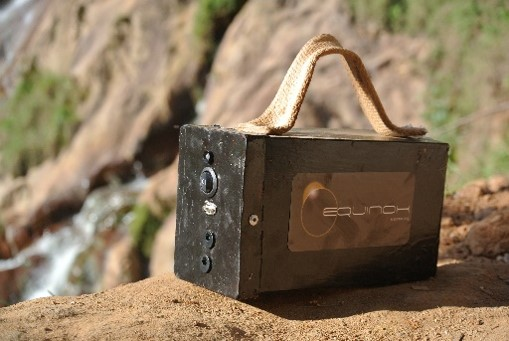
\includegraphics[scale=0.7]{Images/AmaziBox.jpg}
\caption{First Generation e.quinox Battery Boxes deployed at Rugaragara Falls Kiosk}
\label{fig:AmaziBox}
\end{figure}

\begin{figure}[h!]
\centering
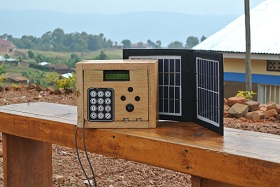
\includegraphics[scale=3]{Images/standalone_box.jpg}
\caption{First Generation Izuba.Box deplyed in Minazi, Northern Rwanda}
\label{fig:IzubaBox}
\end{figure}

Consumers from local community pay to hire the battery boxes under one of two payment schemes: pay-per-recharge and pay-per-month \cite{e.quinox-Hydro-web:2012}. The biggest difference between the two schemes are that users can recharge as often as they would like with pay-per-month. Both payment schemes involve the recharge of the boxes at the energy kiosk when they are depleted of energy.

\subsection*{Standalone Solution}
The Standalone Solution is an independent electrification solution which was recently developed by e.quinox for customers who live far from energy kiosks.

The Stand-alone solution consists of a pay-as-you-go solar electricity generation and storage kit, known as the Izuba.Box \cite{e.quinox-Standalone-web:2012}.  With the Izuba.Box, customers no longer have to travel regularly back to the Energy Kiosk for electricity. Solar panels are installed on the customer's roof, and is connected to a sealed box which contains a large battery box. The attached large battery box allows a regulated power output and access to electricity during dark hours. 

With the customers not returning to Energy Kiosks, the battery boxes are not hired out like the battery boxes are. The high capital costs of the independent solar system is spread over typically a two year rent-to-own payment plan using a mobile payment system.

It is hoped that the Standalone Solution and additional generation from the Energy Kiosk can be complemented the battery boxes in circulation to provide a continuous access to electricity to all households in the village.

\subsection*{Micro-Grid}
With the recent completion of a hydro-electric kiosk, e.quinox for the first time has a kiosk with access to an always-on generator. However, a limited number of battery boxes in circulation and a constant generation available during the off-peak hours leaves an excess capacity for electricity generation. To improve utilisation of the generator in the kiosk, e.quinox has recently started conducting a feasibility study into constructing a transmission line and a distribution network which will serve a village near the kiosk with a view to make the most of the electricity generated.

Preliminary surveys conducted in the nearest village to the kiosk indicates the demand could exceed the amount of excess power generated by the kiosk, making it an ideal scenario for this project. The result of this project can be used in conjunction with other e.quinox feasibility studies to implement a novel type of Micro-Grid with compulsory demand side management. 

\section*{Rugaragara Falls as a Simulation Scenario}
In developing countries such as Rwanda, poor communities with no access to grid electricity are often in isolated locations such as Rugaragara Falls. The local District Sector office estimates that Grid electricty access won't be available in Rugaragara before 2020. In the case of Rugaragara Falls and much of rural Rwanda, the terrain and underdeveloped transport links make fuel expensive to obtain. Therefore instead of non-rewable sources of generation, locals often depend on renewable sources of electricity such as solar and wind. However, renewable generation can be highly variable in the amounts of electricity that is produced due to external factors such as weather, time of day and the season. Without access to redundancies received from the national electricity grid, it can be beneficial for Prosumers within these areas to form a micro-grid to reduce the generation requirement of individual households for continuous electricity access.

%As an example, many people still choose to use battery boxes provided by e.quinox, which is cheaper than connecting to the grid.

% \subsection{Additional Research}
% e.quinox in Rwanda only presents us with one scenario. Additional research is required for other regions such as South America and the Indian Subcontinent to look at potential new scenarios and use cases for various generators and electrical appliances.

% The information above only outlines the existing infrastructures in place. Additional work needs to be done to obtain relevant usage data from e.quinox customers and other electricity users to accurately build a relevant generation mix and demand model.

% In some regions such as Minazi, e.quinox provides the only source of accessible electricity for the local populace. Data on their usage should be more readily available than some of the other locations in other countries. 